
In this section we look at a few examples of foliations arising from fibrations.

\subsection{Algebraic integrability}

It is a natural question to ask when the leaves of a foliation are algebraic
curves. Examples we have seen are $xdy-ydx$, with leaves $ax+by=0$ for
$[a:b]\in\P^1$, and $pxdy+qydx$ for $p,q\in\N$, with leaves $x^qy^p=c$ for
$c\in\A^1$. Notice that $xdy-ydx=y\cdot d(x/y)$, and
$pxdy+qydx=d(x^qy^p)/(x^{q-1}y^{p-1})$, so these are examples of the following
construction.

\begin{definition}
    Given a rational map $f:X\dashrightarrow C$, where $X$ is a surface and $C$
    is a curve, the relative tangent bundle $T_{X/C}$ defines a foliation on $X$
    which we call a \emph{fibration}. The leaves of this fibration are precisely
    the fibers of $f$, which are algebraic curves.
\end{definition}

% TODO: compute N_F = K_C + Σ(m-1)D where fibers of f are ΣmD

In the converse direction, there is a general statement which can be made:

\begin{proposition}\label{prop:fibration}
    Suppose $(X,\scrF)$ is a foliated surface, such that for a general $x\in X$
    the leaf of $\scrF$ through $x$ is algebraic. Then there exists a rational
    map $X\dashrightarrow Y$ such that $T_{X/Y}$ and $T_\scrF$ are isomorphic on
    a dense open subset of $X$.
\end{proposition}

\begin{proof}[Sketch proof]
    We consider the Hilbert scheme $\Hilb_X$. Tangency to the foliation $\scrF$
    is a condition on subvarieties which cuts out a closed subscheme
    $\calT_{X,\scrF}\subseteq\Hilb_X$. By assumption, the canonical map from the
    universal family $\calU$ over $\calT_{X,\scrF}$ to $X$ is dominant. Since
    $\calU$ is an infinite disjoint union of projective components, by the Baire
    category theorem we have some such component $Z\subset\calU$ over
    $Y\subset\calT_{X,\scrF}$ which maps surjectively to $X$. After restricting
    to a suitable hyperplane $Y^0$ in $Y$, we get a finite surjection
    $Z^0\to X$, which lifts to a Galois covering $\tilde Z^0\to X$, where the
    Galois group $G$ can be made to act on a base $\tilde Y^0$.
    \begin{equation*}
        \begin{tikzcd}
            \tilde Z^0 \ar[d] \ar[r]
                \ar[rrr,bend left,"\text{Galois}"] &
            Z^0 \ar[d] \ar[r,hook] &
            \calU \ar[d] \ar[r] & X \\
            \tilde Y^0 \ar[r] & Y^0 \ar[r,hook] & \calT_X
        \end{tikzcd}
    \end{equation*}
    At this point we can collapse the fibers by taking the quotient
    $\tilde Z^0/G$, which maps birationally to $X$, and so we get a rational map
    $X\dashrightarrow \tilde Y^0/G$ which by construction has fibers tangent to
    $\scrF$.
\end{proof}

% TODO expand on Galois coverings, expand on hyperplane section argument

\subsection{Miyaoka's criterion}

We saw in \cref{sec:pencil} an example where $K_\scrF$ being negative forces the
foliation $\scrF$ to consist of rational curves. We present a theorem due to
Miyaoka which asserts a more general result of this form.

% condition = K_F pseff?

\begin{theorem}[Miyaoka]
    Suppose $(X,\scrF)$ is a foliated surface, and $H$ is an ample divisor on
    $X$ such that $K_\scrF\cdot H<0$. Then there is a birational morphism
    $\tilde X\to X$ and a fibration $f:\tilde X\to C$ such that the general
    fiber of $f$ is rational, and $\scrF$ is the foliation induced by $f$.
\end{theorem}

\begin{proof}[Proof (Bogomolov, McQuillan)]
    By Bertini's theorem, for $n\gg0$ we have some smooth curve $C\in|nH|$ which
    is disjoint from $\Sing(\scrF)$. Write $Y=X\times C$, and consider the rank
    1 foliation $\scrG$ on $Y$ given by $\scrF$ on each fiber. The diagonal
    $D\subset C\times C\subset Y$ is disjoint from $\Sing(\scrG)$, and
    integrating $\scrG$ at the points of $D$ gives a local analytic surface $V$
    through $D$.
    \begin{figure}[H]
        \centering
        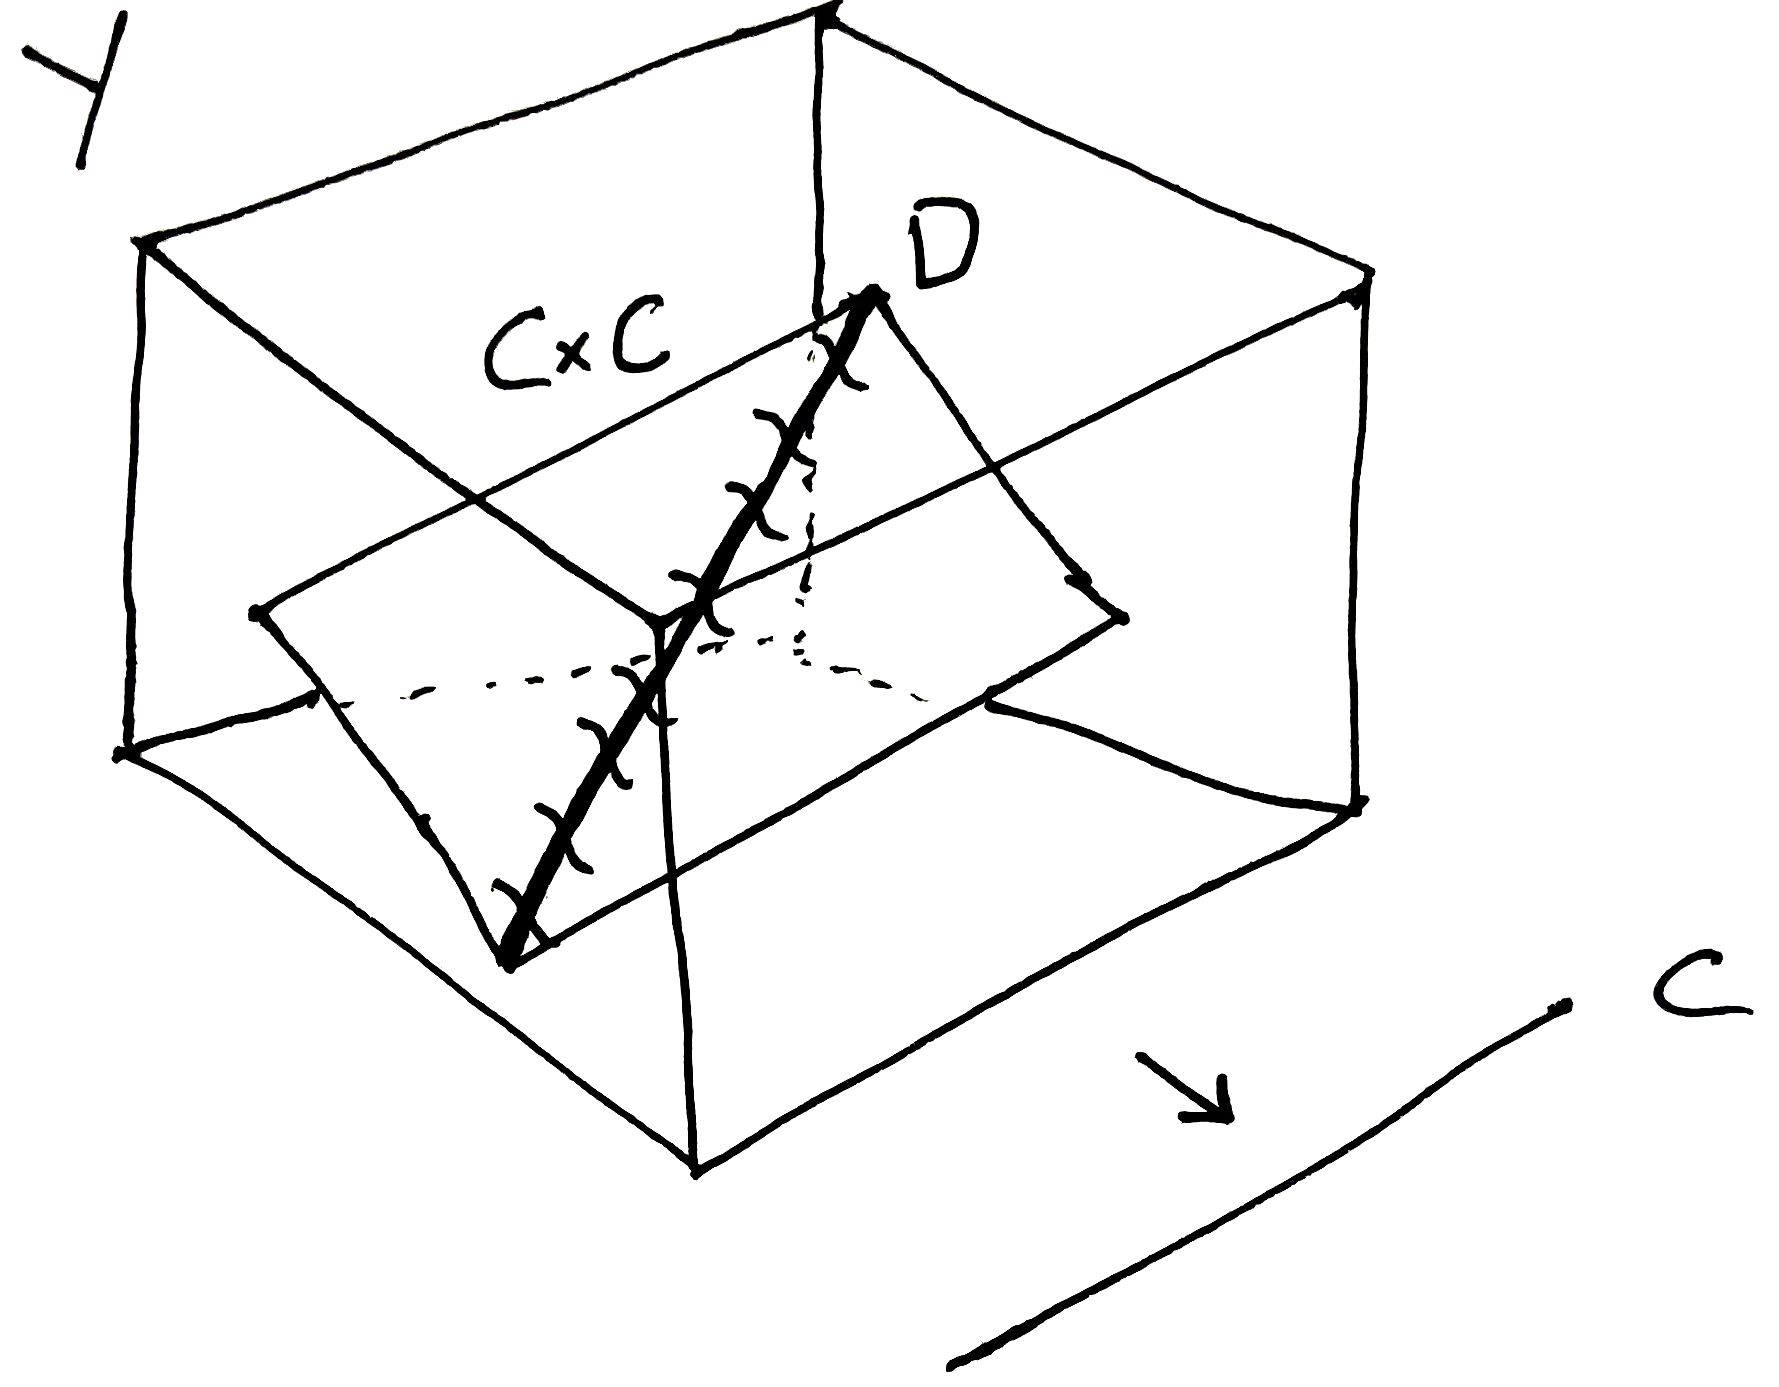
\includegraphics[scale=0.08]{miyaoka} % TODO: white out
        \caption{The foliation $\scrG$ near $D$.}
    \end{figure}
    By construction $N_{D/V}=T_\scrG|_D$, which is identified with $T_\scrF|_C$,
    so $\deg N_{D/V}=T_\scrF\cdot C=nT_\scrF\cdot H>0$. Hence $N_{D/V}$ is
    ample, and this forces the surface $V$ to be algebraic by a theorem of
    Andreotti; see \cite[Thm 3.4]{bost_13}. Write $S$ for its Zariski closure.
    We have shown that the leaves of $\scrG$ through $D$ are algebraic, and
    hence the leaves of $\scrF$ are algebraic. By \cref{prop:fibration} this
    means that $\scrF$ is induced by a fibration, and it suffices to show that
    the general fiber is rational.

    We have a fibration $f:S\to C$, inducing a foliation $\scrH$ on $S$ which
    agrees with $\scrG$ locally around $D$. The fibers of $f$ are reduced, so
    $K_\scrH=K_{S/C}$. Now by Fujita semipositivity, if the general fiber is not
    rational then $K_{S/C}$ is a sum of a nef divisor and an effective disivor,
    and in particular $K_{S/C}$ is nef. But
    $K_{S/C}\cdot D=K_\scrH\cdot D=K_\scrF\cdot C<0$, so the general fiber must
    be rational. Since the fibers of $f$ correspond to the leaves of $\scrF$, we
    are done.
\end{proof}

\begin{remark}
    The condition in this theorem is necessary; suppose $f:X\to C$ is a
    fibration inducing a foliation $\scrF$ whose general fiber is rational. Then
    $K_\scrF=K_{X/C}-D$ where $D\ge0$ is supported on fibers of $f$. If $F$ is a
    general fiber, then $K_\scrF\cdot F=K_X\cdot F=-2$, and $F$ is nef. Hence if
    $H$ is ample we have that $nF+H$ is also ample for $n\ge0$, and
    $K_\scrF\cdot(nF+H)=-2n+K_\scrF\cdot H$ is negative for $n\gg0$.
\end{remark}
